\documentclass[12pt,a4paper]{book}
\usepackage[utf8]{inputenc}
\usepackage[pdftex]{graphicx}
\usepackage[italian]{babel}
\usepackage{fixltx2e,bold-extra,geometry,
    amssymb,amsmath,mathtools, microtype,url,cite}
\usepackage[bookmarks=true, hidelinks, pdftitle={
SELEZIONE DI TOPOLOGIE D'ANTENNA MINIATURIZZATE SU MD},
pdfauthor={Alex Pacini}]{hyperref}
\usepackage{bold-extra}

\pagestyle{headings}
\graphicspath{{images/}}

%%%%%%%%%%%%%%%%% New Commands %%%%%%%%%%%%%%%%%%%%%%%%%%%%%%%%%%%%%%%%%%%%%%%%%
%
\newcommand{\intentblankpage}{
%     Leaves a blank page
    \newpage
    \null
    \vfill
    \thispagestyle{empty}
    \begin{center}
%         \textit{This page intentionally left blank.}
        \textit{Questa pagina \`e lasciata intenzionalmente bianca.}
    \end{center}
    \newpage
}
% 
% Writes intentionally blank page when there is a \newpage on the left page of
% a book.
\makeatletter
    \def\cleardoublepage{\clearpage%
        \if@twoside
            \ifodd\c@page\else
                \vspace*{\fill}
                \hfill
                \begin{center}
%                     \textit{This page intentionally left blank.}
                    \textit{Questa pagina \`e lasciata intenzionalmente bianca.}
                \end{center}
                \thispagestyle{empty}
                \newpage
                \if@twocolumn\hbox{}\newpage\fi
            \fi
        \fi
    }
\makeatother
%
% Length to set margins for 65 chars
\newlength{\sixtyfivecharwidth}
\settowidth{\sixtyfivecharwidth}{
    \normalfont abcdefghijklmnopqrstuvwxyzabcdefghijklmnopqrstuvwxyz1234567890123}
% 
%Integral with the limit below(mathrlap)
% \newcommand{\intlimr}[1]{\ensuremath{\int \limits_{\mathrlap{#1}}}}
% 
% This redefine could cause big issues! See: 
% http://tex.stackexchange.com/questions/248421/use-mathclap-as-default-in-limits-of-integration
% \let\oldlimits\limits
% \def\limits_#1{\oldlimits_{\mathclap{#1}}}
\def\mclimits_#1{\limits_{\mathclap{#1}}}
%%%%%%%%%%%%%%%% End New Commands %%%%%%%%%%%%

\begin{document}
    \pagenumbering{Roman}
    % \newgeometry{margin=26mm} % allarga la pagina anche in altezza
\newgeometry{lmargin=21mm,rmargin=21mm}
\begin{titlepage}
\begin{center}
    
\includegraphics[scale=0.35]{logo.png}\\
    \vspace{8mm}
    {\huge{\textsc{\textmd{Università degli studi di Udine}}}}\\
    \vspace{10mm}
    {\large{\textbf{ Dipartimento di Scienze Matematiche, Informatiche e Fisiche}}}\\
    \vspace{0.5cm}
    {\large{\textbf{ Corso di laurea in Tecnologie Web Multimediali}}}
\end{center}
\vspace{10mm}
\begin{center}
    {\LARGE\textbf{\textsc{Progettazione e sviluppo di}}}\\
    \vspace{6mm}
    {\LARGE\textbf{\textsc{un'applicazione per la}}}\\
    \vspace{6mm}
    {\LARGE\textbf{\textsc{fidelizzazione e il rewarding}}}\\
    \vspace{6mm}
    {\LARGE\textsc{\textbf{degli utenti}}}\\
    \vspace{10mm}
\end{center}
\vfill
\par
\noindent
% \begin{minipage}[t]{0.47\textwidth}
%     \vspace{10mm}
%     \thinspace{\large{\sc Relatore}\\
%     \vspace{2mm}
%     {\bf Prof. STEFANO BURIGAT}}
% \end{minipage}
% \hfill
% \noindent
% \begin{minipage}[t]{0.47\textwidth}\raggedleft
%     \vspace{10mm}
%     {\large{\sc Laureando}\\
%     \vspace{2mm}
%     {\bf RICCARDO CARANFIL}}
% \end{minipage}

\begin{minipage}[t]{0.47\textwidth}
    \vspace{13mm}
    \large{\sc Relatore}\\
\end{minipage}
\hfill
\noindent
\begin{minipage}[t]{0.47\textwidth}\raggedleft
    \vspace{13mm}
    \large{\sc Laureando}\\
\end{minipage}

\begin{minipage}[t]{0.47\textwidth}
    \large\bf{Prof. STEFANO BURIGAT}
\end{minipage}
\hfill
\begin{minipage}[t]{0.47\textwidth}\raggedleft
    \large\bf{RICCARDO CARANFIL}
\end{minipage}

\vspace{18mm}
\begin{center}
    % {\large{\sc I Appello - I Sessione}
    {\rule[0.2cm]{5cm}{0.3mm}\\
    %inserire il numero della sessione in cui ci si laurea
    \large{\sc{Anno Accademico 2018/2019}}}
    %inserire l'anno accademico a cui si è iscritti
\end{center}
\end{titlepage}
\restoregeometry

    \intentblankpage
    
    \newgeometry{text={\sixtyfivecharwidth,35\baselineskip}}
    \vspace*{50mm}
    %\begin{flushright}
    %     {\Large{\bf Keywords:}\\ \vspace{5mm}
    %         Magneto-Dielettrico\\ \vspace{2mm}
    %         Correnti Superficiali\\ \vspace{2mm}
    %         Topologie di Antenne\\ \vspace{2mm}
    %         Far-Field\\
    %     }
    % \end{flushright}
        
    \vspace*{50mm}
    \begin{flushright}
        \textit{\large Ringrazio la mia famiglia e \\ tutti i miei amici per avermi accompagnato lungo questo percorso}
    \end{flushright}
    
    \newpage
    
    \vspace*{30mm}
    \begin{flushright}
        \textit{\large Citazione 
            \\ \vspace{5mm}  - Tizio Caio -}
    \end{flushright}
    
    \vfill
    
    \noindent \hspace{20mm} \textit{\large{Ringraziamenti:}} \vspace{5mm}\\
    Da scrivere
    
    \newpage
    \tableofcontents
    
    \chapter*{Introduzione}
    \pagenumbering{arabic}
    \addcontentsline{toc}{chapter}{Introduzione}  
    \normalsize
L’obiettivo principale del tirocinio presso \textbf{Urbana Smart Solutions srl}\cite{urbanasmartsolutions}
è stata la creazione di un'applicazione
iOS denominata \textbf{QIX} atta alla fidelizzazione e al rewarding di un target di utenti specifico. 
Il principali target di clienti a cui mira l'applicazione sono delle FMCG\footnote{Fast Moving Consumer
Goods}, ossia delle compagnie che vendono beni di consumo a basso
costo e molto velocemente.

Tali compagnie attraverso i loro prodotti possono creare diverse
tipologie di eventi e gli utenti dell’applicazione possono accedervi
e vincere dei punti denominati \textbf{QIX coins} con cui comprare o avere degli
sconti sui beni venduti.

% Esistono diverse modalità in cui un utente può accadere a tali eventi:
% \begin{itemize}
%     \item Usando la funzione “shake” dello smartphone in determinati contesti;
%     \item Usando specifiche funzioni come la G'morning Challenge o la ruota della fortuna;
% \end{itemize}

L’elemento cardine dell’app è il \textbf{QIX Shake} ossia l’attivazione di un particolare servizio
che dipende dal contesto attuale dell'utente e il tipo di offerta che viene selezionata.
Tale servizio dà agli la possibilità di vincere dei QIX coins agitando lo smartphone.
I principali servizi di shake dell'applicazione sono:

\begin{enumerate}
    \item\textbf{TV Shake}: agitando lo smartphone inizierà un'analisi dei dati del microfono
    allo scopo di trovare un particale \textbf{watermark} inserito in campagnie publicitarie televisive;
    \item\textbf{Read Shake}: all'utente viene proposta la lettura di contenuti o questionari in cambio di QIX coins;
    \item\textbf{Video Shake}: a seguito della visualizzazione di uno video l'utente viene premiato con dei punti;
    \item\textbf{Scan shake}: dopo aver scannerizzato il barcode di un prodotto (Es. al supermercato) all'utente verrano assegnati dei punti;
    \item\textbf{Receipt Shake}: dopo aver scannerizzato uno scontrino di acquisto di prodotti partner delle FCMG;
    \item\textbf{Stadium Shake}: inierà anche in questo caso l'analisi del suono esterno per la ricerca di eventuali watermark
    generati in un'audio durante delle partite allo stadio;
\end{enumerate}


    \intentblankpage
    
    \chapter{Formulazione teorica}
    \label{CH:Teoria}
    
Il mio compito nello sviluppo dell'applicazione è stato quello 
di creare un prototipo iniziale avendo a disposizione un mock up creato con
proto.io\cite{protoio} e una serie di requisiti essenziali.

\section{Requisiti essenziali}

La base di partenza di QIX sono state delle funzionalità essenziali e 
sonstanzialmente molto difficili da inserire in una versione dell'app già avanzata.
È stati quindi deciso di creare un prototipo di partenza avente i seguenti requisiti:

\begin{itemize}
    \item {
        \textbf{Navigazione dinamica}: L'applicazione deve gestire dei cambiamenti di contesto
        dinamici: dev'essere possibile mostrare all'utente contenuti dinamici indipendentemente
        dal contesto in cui si trova.
    }
    \item {
        \textbf{QIX Shake}: L'utente deve poter agitare lo smartphone in qualsiasi
        sezione dell'applicazione e il risultato deve essere basato sul contesto attuale o su delle direttive dettate
        da delle Rest API;
    } 
    \item {
        \textbf{Animazioni interattive}: L'intera applicazione dev'essere progettata in modo tale da presentare all'utente
        delle \textbf{animazioni interattive} in stile CardView\cite{cardview} disponibili in 
        qualunque sezione o vista in cui si trovi l'utente e definite dal contesto attuale;

        Le animazioni in questione devono essere progettate in pagine, in cui ogni pagina può contenere 
        più CardView. L'utente vedrà in un determinato momento una e soltanto una pagina.

        Ogni CardView deve essere trascinabile dall'utente e deve interagire con le altre CardView della pagine. 
        Quando l'utente usa una forza di trascinamento superiore a un valore di soglia tutte le viste devono
        cadere per gravità;
        
        Tale gravità finirà con la fine dell'animazione o l'apparizione di una nuova pagina se presente;
    }
    \item {
        \textbf{Autenticazione}: L'applicazione deve supportare tre diversi stati o modalità di autenticazione:
        \begin{enumerate}
            \item\textbf{Trial Mode}: l'utente è anonimo, esiste solo un id per tenere traccia dei suoi QIX coins.
            \item\textbf{Signed Mode}: l'utente ha inserito il numero di telefono e il suo genere;
            \item \textbf{Pro Mode}: l'utente aggiunge dei dati su se stesso o collega il suo account a dei social media come Facebook, Google o Instagram;
        \end{enumerate}
        Si nota facilmente che non esiste una stato in cui l'utente non è registrato: questo perchè
        per tenere traccia dei suoi QIX coins e di altri dati utili è necessario avere una riferimento all'utente;
    }
    \item {
        \textbf{DeepLinks}: L'applicazione deve poter essere avviata dinamicamente
        attraverso dei \textbf{Deep Links}\cite{deeplinks};
        E deve essere in grado di gestirli in base al contesto dell'utente;
    }
\end{itemize}

\section{La navigazione dinamica}

% Analizzando il requisito mi sono posto diverse domande: \\ \\
% \noindent{
%     \large\textit{Cosa significa dinamicamente?}
%     \normalsize{Il nostro obiettivo in questo caso è mostrare all'utente \textbf{contenuti diversi}
%     indipendentemente dal constesto e quindi dalla vista in cui si trova}\\ \\
%     \large\textit{Quale contesto?}
%     \normalsize{Con contesto dell'utente si intende lo stato attuale dell'applicazione,
%     quindi l'intero stack di navigazione se presente;
%     } \\ \\
% }

Prima di entrare nel merito della soluzione al problema, elenco brevemente gli
standard di navigazione delle app iOS.

Ogni applicazione può avere degli \textbf{UINavigationController}\cite{navigationcontroller},
ossia dei contenitori di \textbf{UIViewController}\cite{viewcontroller} che vengono
utilizzati per mantenere lo stack di navigazione e gestire la transizioni tra due UIViewController.

Nella figura~\ref{fig:1} si nota facilmente come il Navigation controller gestisce un'array di View Controller e una sola 
navigation bar. 
In iOS sono infatti innate molte animazioni di navigazione che è utile sfruttare, piuttosto di creare 
componenti custom poi difficili da rendere interattivi.\\

\begin{minipage}{\linewidth}
    \centering
    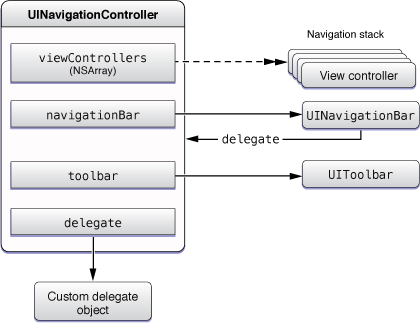
\includegraphics[width=5cm]{navigation}
    \captionof{figure}{Navigation controller scheme}
    \label{fig:1}
\end{minipage}

\subsection{Tipologie di navigazione}\label{sec:navigation}

Esistono tre tipologie base di navigazione:


\begin{enumerate}
    \item{\textbf{Push}: un UIViewController avente un navigation controller può rendere
    visibile un altro ViewController attraverso la funzione "pushViewController" di un Navigation controller\par
    \begin{minipage}{\linewidth}
        \centering
        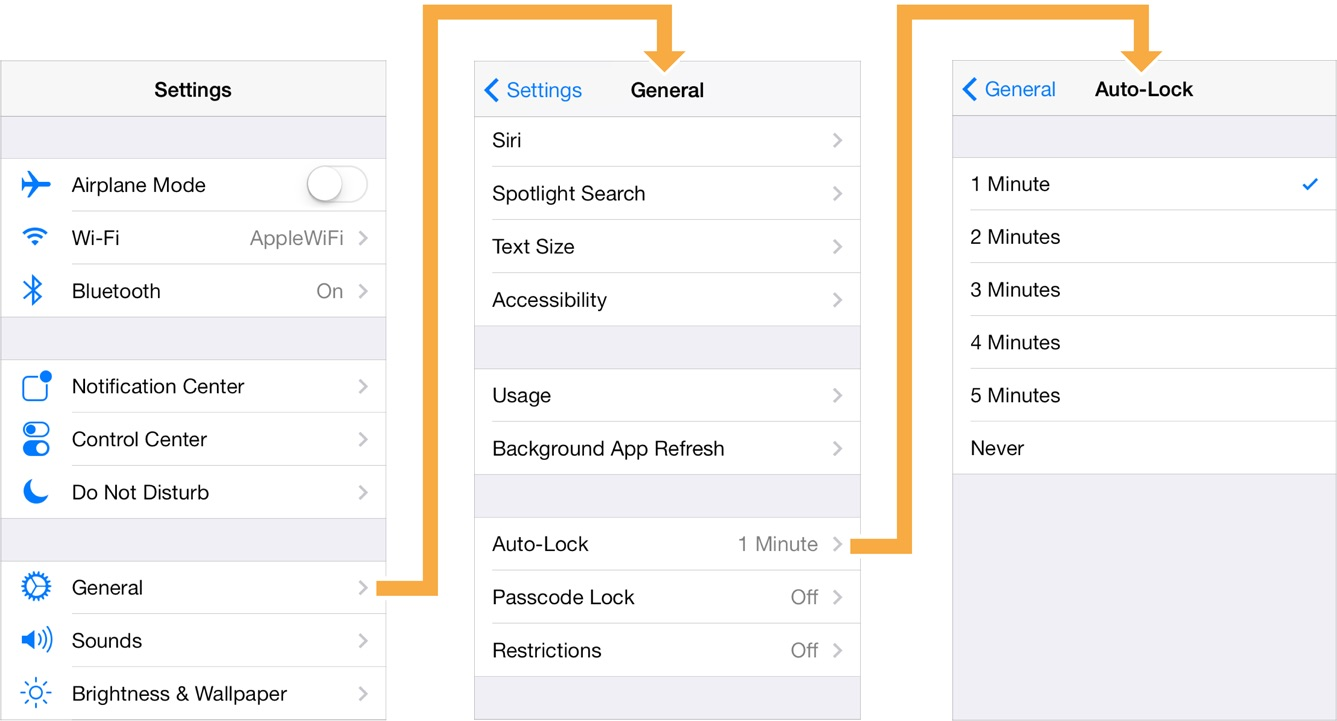
\includegraphics[width=10cm]{push}
        \captionof{figure}{Presantazione di un ViewController tramite push}
        \label{fig:2}
    \end{minipage}
    }
    \item{ \textbf{Modal}: un ViewController può presentare un altro ViewController senza necessariamente avere un 
        Navigation Controller, l'animazione standard è dal basso verso l'alto come in figura~\ref{fig:3}\par
        \begin{minipage}{\linewidth}
            \centering
            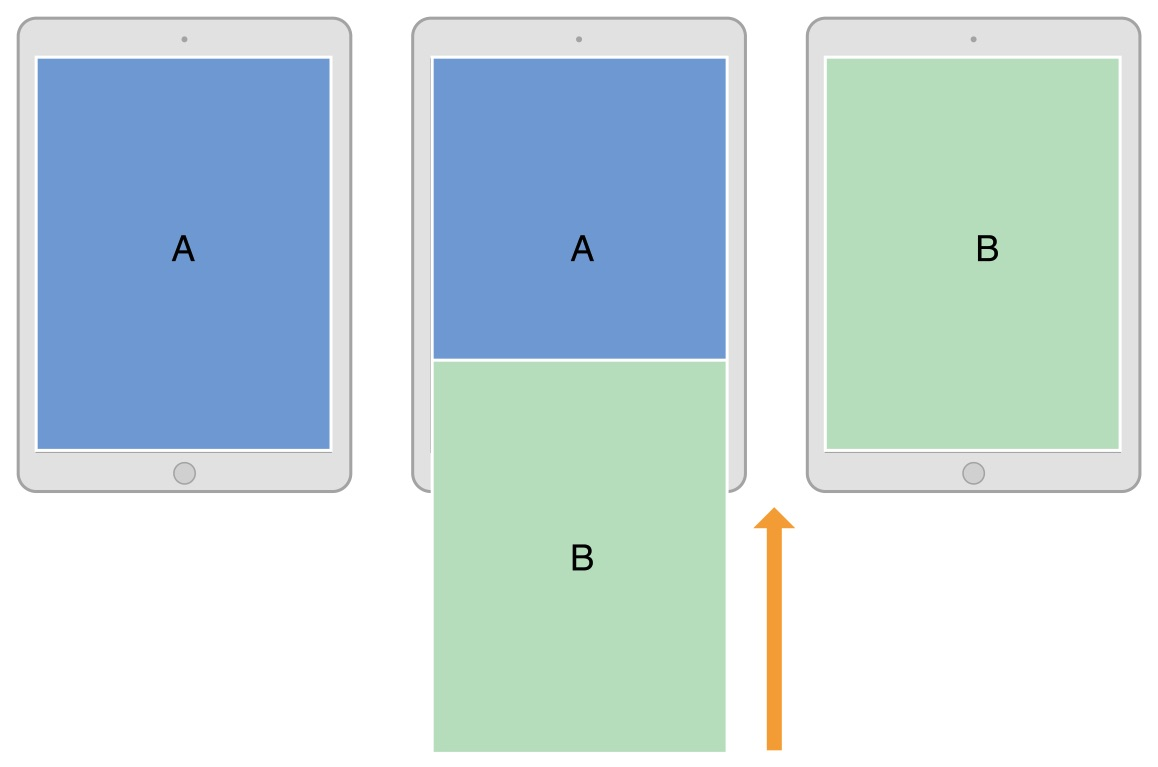
\includegraphics[width=10cm]{modal}
            \captionof{figure}{
                Presantazione di un ViewController tramite modal
            }
            \label{fig:3}
        \end{minipage}
    }
    \item{\textbf{Segue}: Una segue non è altro che un link tra due view controller attraverso un'interfaccia
        grafica. In base alla tipologia cambia il tipo di navigazione (Modal o Push)
    }
\end{enumerate}

Avendo definito i principali metodi di navigatione tra ViewController torniamo al problema iniziale:
\textit{Come possiamo rendere dinamica la navigazione?}

A seguito di uno studio approfondito di varie tecniche di navigazione iOS ho scelto di utilizzare il
\textbf{Coordinator Pattern}\cite{coordinatorpattern}.

\subsection{Il Coordinator Pattern}

Generalmente in iOS l'intera logica di un ViewController viene scritta nel ViewController stesso, creando spesso
file di grosse dimensioni e disordine generale. Il Coordinator Pattern è nato proprio per rendere 
le applicazioni più scalabili e leggere. 

Ogni ViewController infatti delega tutte le decisioni al suo Coordinator che in base a determinate logiche deciderà
i passi successivi.

Ogni Coordinator può controllare un ViewController o più Coordinator, questo rende le viste
indipendenti tra di loro e rende ogni ViewControler totalmente invisibile agli altri.\\

\begin{minipage}{\linewidth}
    \centering
    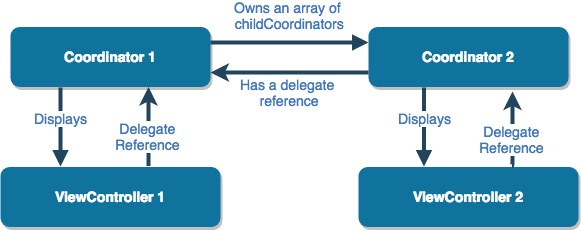
\includegraphics[width=10cm]{coordinator}
    \captionof{figure}{
        Il Coordinator Pattern
    }
    \label{fig:4}
\end{minipage}\\ \\

La resposibilità dei coordinator è infatti la navigazione, come un navigation controller gestisce i sui View Controller, un coordinator gestisce
i suoi figli e questo rende ogni vista o flow di navigazione totalmente indipendente dal resto dell'applicazione.

Per navigare tra i view controller vengono generalmente usate le tipologie di navigazione
descritte nella sezione~\ref{sec:navigation}, tranne le segue, che essendo definete da vista grafica renderebbero
la navigazine statica e fissata su determinati ViewController. \\


Di seguito in figura~\ref{fig:5} presento uno schema dell'utilizzo di due coordinator
per la gestione di una lista di prodotti e il carrello. \\

\begin{minipage}{\linewidth}
    \centering
    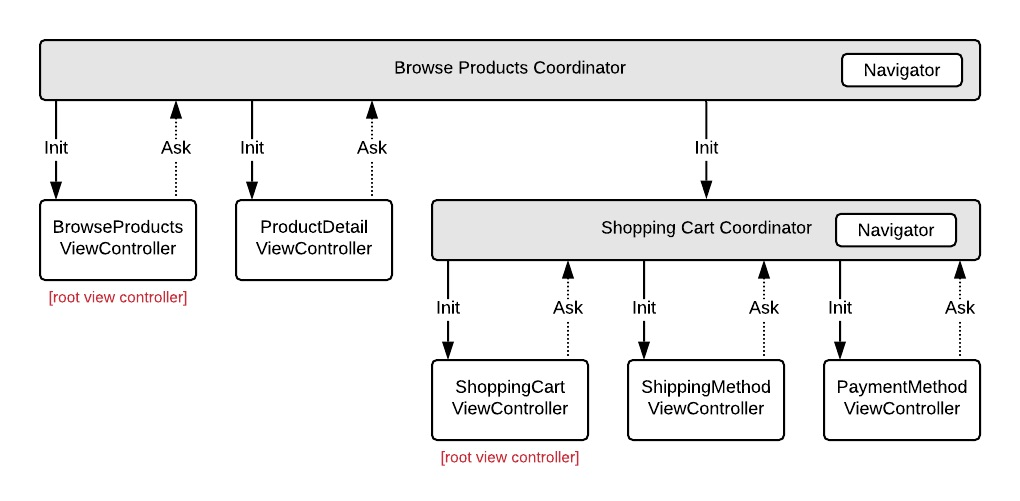
\includegraphics[width=10cm]{coordinator-example}
    \captionof{figure}{
       Esempio di coordinator pattern
    }
    \label{fig:5}
\end{minipage}\\ \\

Come si evince dall'immagine è presente in entrambi i coordinator è presente un oggetto
\textbf{navigator} che sarà in gestore di un UINavigationController

\section{Il QIX Shake}

In iOS ogni UIViewController risponde a degli eventi. L'evento designato per lo shake è
\begin{minted}{swift}
    func motionEnded(_ motion: UIEvent.EventSubtype,
        with event: UIEvent?)
\end{minted}

In caso di shake infatto motion sarà uguale a .motionShake
Per rendere disponibile l'evento "shake" in un qualunque ViewController la soluzione è stata abbastanza semplice:
è bastato l'utlizzo di un ViewController Genitore e attrvaerso l'eriditarietà ogni view controller è in grado
di eseguire la stessa funzionalità.

In questo caso è stato optato l'utilizzo delle notifiche locali: quando avviene uno shake i view controller inviano una notifica 
globale e solo gli observer vi hanno accesso.

\section{Le animazioni interattive}


    
    \chapter{Validazione numerica}
    \label{CH:Val_num}
    \input{./capII}
    
    \chapter{Conclusioni}
    \label{CH:Concl}
    % Lo sviluppo di QIX è stata una delle esperienze più formative della mia carriera
% studentesca e professionale. Ci sono state molte difficoltà tra cui irequisiti non sempre chiari e
% la complessità dell'applicazione, che mi hanno però sempre spinto a imparare sempre di più e non darmi per viewcontroller.
% Il futuro vede in QIX un'applicazione 
Il mio compito in QIX è stato progettare e implementare, insieme ad un intero team di sviluppo, 
l'applicazione QIX basandosi su dei requisiti base definiti dal team a seguito di molti meeting 
e brain storming. L'applicazione è ancora agli inizi, una prima versione potrebbe già essere.
negli store questo inverno.
    
    \chapter{Riconoscimenti}
    \label{CH:Ric}
    \input{./riconoscimenti}
    
%     \nocite{*}
    \bibliographystyle{IEEEtran}
    \bibliography{myworks,books,journals,conferences,others}
    
    \listoffigures
\end{document}
